
%(BEGIN_QUESTION)
% Copyright 2006, Tony R. Kuphaldt, released under the Creative Commons Attribution License (v 1.0)
% This means you may do almost anything with this work of mine, so long as you give me proper credit

Calculate the proper LRV and URV pressures for the 4-20 mA loop-powered $\Delta$P transmitter in this level measurement scenario:

$$\includegraphics[width=15.5cm]{i00520x01.eps}$$

\begin{itemize}
\item{} LRV = \underbar{\hskip 50pt} inches water column
\vskip 10pt
\item{} URV = \underbar{\hskip 50pt} inches water column
\end{itemize}

Then, calculate the transmitter's output given the following process levels (assuming perfect transmitter calibration):

\begin{itemize}
\item{} Output = \underbar{\hskip 50pt} mA with the kerosene level 4 feet up from the bottom of the tank (4 feet ``fillage'')
\item{} Output = \underbar{\hskip 50pt} mA with the kerosene level 6 feet down from the top of the tank (6 feet ``ullage'')
\end{itemize}

\vskip 20pt \vbox{\hrule \hbox{\strut \vrule{} {\bf Suggestions for Socratic discussion} \vrule} \hrule}

\begin{itemize}
\item{} Suppose the DP transmitter with the remote seal failed and had to be replaced.  Unfortunately, you don't have another DP transmitter with a remote seal in stock to replace it.  Could you use a DP transmitter {\it without} a remote seal for this application?  If so, would its calibration have to be different from the remote-seal transmitter?
\item{} Explain why this installation does not require a {\it compensating leg}.
\end{itemize}

\underbar{file i00520}
%(END_QUESTION)





%(BEGIN_ANSWER)
 
Note: a weight density ($\gamma$) of 51.2 lb/ft$^{3}$ is assumed for kerosene.

\begin{itemize}
\item{} LRV = \underbar{\bf 56.62} "WC = 2.046 PSI
\item{} URV = \underbar{\bf 164.9} "WC = 5.959 PSI
\end{itemize}

\begin{itemize}
\item{} Output = \underbar{\bf 5.455} mA with the kerosene level 4 feet up from the bottom of the tank (4 feet ``fillage'')
\item{} Output = \underbar{\bf 12.73} mA with the kerosene level 6 feet down from the top of the tank (6 feet ``ullage'')
\end{itemize}

%(END_ANSWER)





%(BEGIN_NOTES)


%INDEX% Measurement, level: hydrostatic pressure

%(END_NOTES)


